\documentclass[a4paper, 12pt]{article}
\usepackage[a4paper,textwidth=170mm,textheight=245mm]{geometry}

\usepackage[utf8]{inputenc}
\usepackage{todonotes}
\usepackage{amsmath}
\usepackage{parskip}
\usepackage{listings}
\usepackage{float}

\begin{document}
\date{}

\title{\Large Classy: Feature Evaluation using Naive Bayes for Genre Classification}

\author{
{Michael Sörsäter}\\
IDA Linköping
}

\maketitle

% Use the following at camera-ready time to suppress page numbers.
% Comment it out when you first submit the paper for review.
%\thispagestyle{empty}

\subsection*{Abstract}
Your Abstract Text Goes Here.  Just a few facts.
Whet our appetites.

\section{Introduction}
Music is a big part of our modern society.
According to Spotify, during 2017 I personally listened to over 60 000 minutes of music.
As everything else in our world we order things and place them in different categories.

Music is often categorized in large genres like \textit{pop}, \textit{rap} and \textit{rock} and is in turn categorized further, like \textit{indiepop}, \textit{dream pop} and \textit{synth pop}.
The most defining features of a genre is the sound, which instruments is used, the tempo, and the structure of the song like number of Verses and Choruses.
Even if the sound have the greatest impact when deciding a genre the lyrics tend to follow certain patterns.

I think that pop music generally tend to be about love and easier subjects whereas rap usually have more complex language and have a more storytelling structure.

In this project a classifier will be implemented to determine the genre of songs.
Different features will be considered to classify the genres and will be evaluated to see if they improve the result or not.
A lot of focus will lie on comparing the two genres pop and rock but also on all 6 genres.

\section{Teory}
The Naive Bayes classifier is commonly used for music classification and have shown in previous work to be an effective model for document classification. \todo[inline]{referenser}

\subsection{Naive Bayes}
Naive Bayes build a probabilistic model that uses arbitrary features from documents.
When training the model features are extracted for different documents and are feeded to the model together with the document class.
For each feature and class the probability in formula \ref{eq:feat} is calculated where $ feat_{i}$ is feature i and $ class_k $ is class k.

\large
\begin{equation}
    p (feat_{i}|class_{k})
    \label{eq:feat}
\end{equation}
\normalsize

When predicting the class of a document the same features are extracted and given to formula \ref{eq:bayes} where there exist $K$ classes and $n$ features for each document.
The probability of the class is multiplied by all features explained in formula \ref{eq:feat}.
The predicted class is the one with highest probability.

\large
\begin{equation}
    \hat{y} = \underset{k \in \{1,2,...,K\}}{argmax} \, \, \, p(class_{k}) \prod_{i=1}^{n} p (feat_{i}|class_{k}
    \label{eq:bayes}
\end{equation}
\normalsize

The strength of the Naive Bayes classifier is that the features are arbitrary.
The model determine the importance for all features and let informative features influence the prediction a lot as well as assign uninformative features with low probabilities.danc

\section{Data set}
\label{sec:dataset}
The acquisition of a good data set is a task that requires careful consideration.
Usually one artist (will use the word artist for artist/band/group) are labeled with just one genre and all songs produced by that artist are assumed to be that genre. \todo{länka till det fam}
This assumption can result in a lot of bad classification as one artist is not bound to one genre.
Previous obtained data sets were considered.
The problem with copywriting often have the impact that bag of words model are used where the different words are coverted to integers. \todo{ref-million song dataset}
This representation makes it hard to work with the models and to evaluate the result.
Many data sets found had not been classified with genres or had to many genre classes in them.
For these reason I made the decision to create my own corpus.

When the data set was created three steps were followed.
Firstly, getting lists of tracks tagged with their genre.
Secondly, from the name of the tracks, get an url to a webpage hosting lyrics.
Thirdly, from the urls, scrape and store the lyrics.

\subsection{List of tracks}
Across the internet it exist a lot of different lists of songs in different genres.
The following criterias were considered when looking for lists of tracks:
\begin{itemize}
    \item {\textbf{Organization} - lists made by individuals can be subjective and is avoided. Lists by organizations tend to be more thought through.}
    \item {\textbf{Reliable} - the producer behind the list should have a lot of experience and knowledge about music.}
    \item {\textbf{Genre cover} - the different genres should come from the same source. Many lists of just \textit{rap} or \textit{electronic} exist but are produced by different persons/organizations.}
    \item {\textbf{Few genres} - because of limitations in the project scope and computational power just a few genres should be included. The goal was to have at top around 5 different genres.}
    \item {\textbf{A lot of data} - to get a reliable model at least a couple of hundred songs is needed in each genre}
\end{itemize}

I found that billboard fulfills all these criterias.

Billboard is a music magazine that was founded in 1894.
Since then billboard have been an important organization in the music industry.
Each year they release lists of the topmost tracks in different categories.
Among other lists they have lists for the genres \textit{pop}, \textit{country}, \textit{rock}, \textit{r\&b/hip-hop}, \textit{rap} and \textit{dance/electronic}.
\todo{https://www.billboard.com/charts/year-end}

For the different lists, there is data from the latest 5-10 years which makes a decent amount.
By going through these webpages with lists and scraping the data the corpus was created.

Some lists were missing so I used Wayback Machine \todo{länka till det kanske?} to retrieve some data and also found a missing list in a forum.

From the lists the name of the artist, song and genre were saved and duplicates were removed.
If there existed several copies within the same genre only one was saved.
Duplicates within the same genre comes from that many lists are similar to each other or that songs are on top lists for multiple years.
If one song was labeled with more than one genre, all occurences of that song were removed.
From all lists the total number of songs were around 6000.
After removing duplicates within the same genre around 4200 remained and after removing songs in more than one genre 3271 were left.

The songs sorted by genre can be found in table \ref{tab:distribution}.

\begin{center}
\begin{table}[h]
    \centering
    \begin{tabular}{| l | r |}
    \hline
    Genre & Count \\ \hline
    total & 3271 \\
    pop & 700 \\
    rap & 322 \\
    rock & 613 \\
    electronic & 389 \\
    country & 423 \\
    r\&b & 824 \\ \hline
  \end{tabular}
  \caption{Genre distribution in corpus}
  \label{tab:distribution}
\end{table}
\end{center}

The tracks are saved in a json file with key an integer counter and value artist, title and genre.

\subsection{Match tracks with urls}
From the name of the tracks the Genius API was used to find the urls. \todo{ref genius}

Using the API a search query was sent with the artist and title in it.
The API returned the matches for the search query.
If the artist and title had an exact match the url was returned.

During this process there were a lot of variantions on the spelling so if the Levenshtein distance between the names were less than 2 they were considered a match.
For the tracks that didn't have a match, the alternatives the search query returned were given to the user.
By entering the index for the correct alternative the url was returned.

For some tracks the Genius API didn't found the correct song and for these the urls were found by hand.

The linking between track and url is made in a separate json file which makes it possible to use another project file where the tracks belong to other genres.

\subsection{Scrape lyrics}
From the json file with the tracks and urls all urls were retrieved from Genius.
Their API does not support to get the lyrics so regular scraping was used with \textit{requests} and \textit{Beautiful Soup}. \todo{länkar}
The lyrics was stored in files named artist + title.

\section{Method}
As mentioned in section \ref{sec:dataset} the data set was created by scraping lyrics from Genius by using lists obtained from billboard.

When the data was in place the classifier was created.
The library nltk for Python3 was used in this project. \todo{citera nltk}
For the classifier, a class was created that is based on the class ``NaiveBayesClassifier'' found in nltk.

When running the classifier a project file is required.
From the project file the corpus is created.
The corpus exist of the lyrics together with the true genre.
When the corpus is created it is shuffled.
The seed for the random function is initialized with a constant value to ensure reproducibility.

\subsection{Baseline}
\label{sec:baseline}
The classifier is initialized with the shuffled corpus and the data is split up in train data and test data.
The default values are that $70\%$ are train and $30\%$ are test data.
Preprocessing of the training data is made to extract all unigrams.
For each song, each line are split by a space and the words are saved.
The most common unigrams are found by sorting all unigrams by their frequencies and the topmost 2500 are stored.

For each song in both the training data and test data the unigrams are extracted in the same way as in the preprocessing phase.
Each song will have boolean unigram features if the unigrams exist in the most common features or not.

The model is trained by the features in the train data and tested with the features in the test data.
The accuracy is calculated for the test set.
For each genre the precision, recall and f-measure is derived.

\subsection{Features}
In the classifier several features are added and explained in this section.

\subsubsection*{Unigram threshold}
When using all data, the maximum number of unigram features are around 5500 but with so many features the system takes really long to run and the performance is only marginally better.
Therefor the default value is set to around half of the maximum value to 2500.

\subsubsection*{Bigrams and bigram threshold}
The bigrams are extracted in the same way as the unigrams.
The number of bigrams used in the model are settable as well with the default value set to 1000.

\subsubsection*{Meta data}
The lyrics found at Genius sometimes contain metadata about the structure of the songs.
One example is the song \textit{Ed Sherran - Thinking Out Loud}:

\begin{verbatim}
    [Verse 1]
    When your legs don't work like they used to before
    And I can't sweep you off of your feet
    ...

    [Pre-Chorus 1]
    People fall in love in mysterious ways
    Maybe just the touch of a hand
    ...

    [Chorus]
    So honey, now, take me into your loving arms
    Kiss me under the light of a thousand stars
    ...

    [Verse 2]
    ...

    [Pre-Chorus 2]
    ...

    [Chorus]
    ...

    [Chorus]
    ...

\end{verbatim}

This structure, \textit{verse}, \textit{chorus}, \textit{verse}, \textit{chorus}, \textit{chorus} is a typical structure for a pop song.
Other types that are used in the model: \textit{intro}, \textit{outro}, \textit{break}, \textit{bridge}, \textit{skit}, \textit{hook}, \textit{drop}, \textit{interlude} and \textit{breakdown}.
When processing lyrics to extract n-grams the lines that starts and ends with ``[ ]'' are ignored to avoid adding these words to the model.
When the features metadata is added the classifier looks for the types within the brackets.
The number for each type is added as the feature.

\subsubsection*{Stopwords}
With this feature all stopwords are ignored.
Stopwords are often the same independent of the genre.
The stopwords used are the ones found in the nltk library and items in pythons' punctuation found in the library string.

\subsubsection*{Tokenization}
Usually tokenization is made at the beginning when processing documents.
In this baseline system the tokenization is made by hand, as explained in section \ref{sec:baseline}.
This feature utilizes the word tokenization found in nltk instead of manual tokenization.

\subsubsection*{Stem}
In regular text many words are inflected and the basic word, stem, is often the wanted word.
This feature uses the nltk SnowballStemmer to stem the words.

\subsubsection*{Length of lyrics}
The length of the lyrics can be an indication on the genre.
Some electronic songs are usually short and repetative with many parts in the song just music.
Hip\/hop and rap are previously shown to contain longer lyrics and more complex language \todo{https://pudding.cool/2017/02/vocabulary/index.html}.

Three features are added:
\begin{itemize}
    \item {Number of characters}
    \item {Number of words}
    \item {Number of unique words}
\end{itemize}

The features are boolean features.
The feature takes a threshold value that determines the value of the feature.
Finding threshold values are tricky, especially when all genres are included, the difference can be small between too many genres.
When analyzing the counts, normalized histograms are created that are colored by genre.
Figure \ref{fig:words} shows the number of words in all pop and rap songs.

\begin{figure}[H]
    \centering
    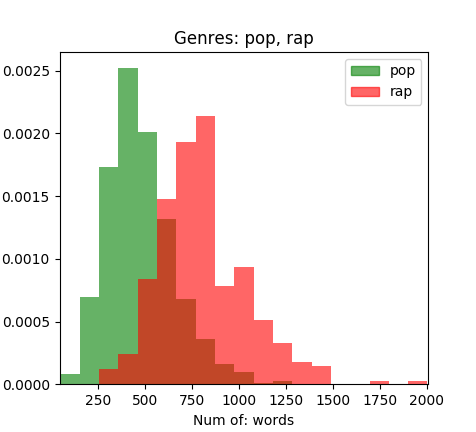
\includegraphics[width=0.7\textwidth]{res/words-pop_rap.png}
    \caption{Number of words in the corpus}
    \label{fig:words}
  \end{figure}

\subsection{Options}
To run and use the system several options are added to the system which are exlained below.

\begin{itemize}
    \item {\textbf{Genres} - Default is to use all genres but can can be changed to any genres that are provided in the project file.
    When testing certain features it is only relevant to have a few number of genres.}
    \item {\textbf{Iterations} - When running a test the data is shuffled and then split up in train and test.
    Between different runs the result can differ so to get reliable result the test need to be run a number of times.
    The number of iterations are determined by this option.}
    \item {\textbf{Split} - In the baseline system the default value to split training and test data is 70 and 30 percent respectively.
    This can be changed with the parameter split.}
    \item {\textbf{Count} - }
    \item {\textbf{Show features} - }
    \item {\textbf{Stats} - }
\end{itemize}

\subsection{Code}
During this project a lot of effort was made in making a good and usable system, for both scraping, getting lyrics, use different features and run different tests.
The code can be found at github \todo{länka till git}
Documentation on how to run the system can be found in the repository's ``README''.

\section{Results}
When discussing the resuls

The baseline system is 



The random seed is set to a fix number to be able to reproduce results.

baseline

unigram - th
bigram - b th
meta - data

stopwords

tokenization

stem

length of lyrics


* Presentera baseline
* olika features
\section{Discussion}
What do you make of it? Discuss your results and
present your analysis in terms of the background theory. \cite{Tsaptsinos2017}
\section{Conclusion}
In what sense has your project reached its goal? What
did you learn from your project?
\cite{Canicatti}
\section*{References}
Present a complete list of references. Choose a
bibliographic style and stick to it.


\bibliographystyle{ieeetr}
\bibliography{res/classy}


\end{document}

